\section{Laplacian Algebras and Quotient Calculus}
\label{sec:laplacian-calculus}

\subsection{Laplacian algebras: differential closure and finite generation}
\label{sec:laplacian-foundations}

Following Mendes--Radeschi \cite[Section~5]{MendesRadeschi}, we develop
closure and finite generation to reduce differential calculations to
finite tables and identify the smallest algebra containing a defining polynomial.

Let \(V=\R^N\) have its Euclidean inner product, let \(\R[V]\) be its
ring of real polynomial functions, and put \(R(x)=|x|^2\).
For smooth functions define
\[
 \Gamma(f,g)=\langle\nabla f,\nabla g\rangle.
\]
All polynomial algebras contain the constants; their generators need
not be algebraically independent.

\begin{definition}[Mendes--Radeschi]
\label{def:laplacian-algebra}
A subalgebra \(\cA\subset\R[V]\) is a \emph{Laplacian algebra} if
\(R\in\cA\) and \(\Delta f\in\cA\) for every \(f\in\cA\).
\end{definition}

This definition is orthogonally invariant and requires no group action.

\begin{lemma}[Gradient closure and homogeneity]
\label{lem:laplacian-grading}
A Laplacian algebra is closed under \(\Gamma\) and contains every
homogeneous component of each of its elements. In particular,
\(\cA=\bigoplus_{d\geq0}\cA_d\), where
\(\cA_d=\cA\cap\R[V]_d\) and \(\R[V]_d\) denotes the homogeneous
polynomials of degree \(d\).
\end{lemma}

\begin{proof}
The product rule gives
\begin{equation}\label{eq:Gamma-polarization}
 2\Gamma(f,g)=\Delta(fg)-f\Delta g-g\Delta f.
\end{equation}
Thus \(\Gamma(f,g)\in\cA\) for \(f,g\in\cA\). The Euler operator
\(E=x\cdot\nabla\) consequently preserves \(\cA\), since
\(Ef=\Gamma(R,f)/2\). If \(f=\sum_{j=0}^D f_j\) is its homogeneous
decomposition, then \(Ef_j=jf_j\). For each \(0\leq d\leq D\), choose
the interpolation polynomial \(p_d\) satisfying
\(p_d(j)=\delta_{dj}\) for \(j=0,\ldots,D\). Then
\(f_d=p_d(E)f\in\cA\).
\end{proof}

\begin{example}[Orthogonal invariants]
\label{ex:orthogonal-laplacian}
If a group \(H\subset O(V)\) acts orthogonally, its invariant algebra
\(\R[V]^H\) is Laplacian. Indeed, \(R\) is invariant and
\(\Delta(f\circ h)=(\Delta f)\circ h\) for \(h\in H\).
For compact \(H\), normalized Haar averaging gives
\[
 \Pi_Hg(x)=\int_H g(hx)\,dh,
 \qquad \Pi_H(fg)=f\Pi_H(g)\quad(f\in\R[V]^H).
\]
The projection below extends this module property to every Laplacian algebra.
\end{example}

\begin{example}[Two orthogonal blocks]
\label{ex:two-block-laplacian-background}
Let \(V=\R^p\oplus\R^q\), where \(p,q\geq1\), and write
\(x\in\R^p\), \(y\in\R^q\), \(u=|x|^2\), \(v=|y|^2\). Then \(R=u+v\), and
\[
 \Delta u=2p,\quad \Delta v=2q,\qquad
 \Gamma(u,u)=4u,\quad \Gamma(u,v)=0,\quad \Gamma(v,v)=4v.
\]
For a polynomial \(h(u,v)\), direct differentiation therefore gives \(\Delta h=4u h_{uu}+4v h_{vv}+2p h_u+2q h_v\).
Thus \(\R[u,v]\) is Laplacian, with image \([0,\infty)^2\).
\end{example}

\subsubsection{The Reynolds projection}

We recall the properties needed for finite generation, following
\cite[Lemma~21, Corollary~22, and
Theorem~23]{MendesRadeschi}.

For polynomials \(f,g\) and an integer \(j\geq0\), set
\[
 B_j(f,g)=\sum_{i_1,\ldots,i_j=1}^N
 (\partial_{i_1}\cdots\partial_{i_j}f)
 (\partial_{i_1}\cdots\partial_{i_j}g),
 \qquad B_0(f,g)=fg.
\]
The product rule and commutation of derivatives give
\begin{equation}\label{eq:MR-higher-contraction}
 2B_{j+1}(f,g)=\Delta B_j(f,g)-B_j(\Delta f,g)-B_j(f,\Delta g).
\end{equation}
Induction shows that \(B_j(f,g)\in\cA\) whenever \(f,g\in\cA\).
If \(f\) is homogeneous of degree \(d\), write
\(f=\sum_{|\alpha|=d}f_\alpha x^\alpha\) and define the
constant-coefficient operator
\(f(\partial)=\sum_{|\alpha|=d}f_\alpha\partial^\alpha\).
Counting ordered derivatives gives
\begin{equation}\label{eq:MR-dual-operator}
 f(\partial)g=\frac1{d!}B_d(f,g).
\end{equation}
In particular, \(f(\partial)\) takes \(\cA\) into \(\cA\).

On the finite-dimensional space \(\R[V]_d\), use the Fischer inner
product
\[
 (f,g)_d=f(\partial)g
 =\sum_{|\alpha|=d}\alpha! f_\alpha g_\alpha.
\]
For degrees \(a,b,a+b\), the coefficient formula also gives
\begin{equation}\label{eq:MR-Fischer-adjoint}
 (fg,h)_{a+b}=(g,f(\partial)h)_b.
\end{equation}

\begin{proposition}[Reynolds projection; Mendes--Radeschi]
\label{prop:MR-Reynolds}
Let \(\Pi_d:\R[V]_d\to\cA_d\) be orthogonal projection for the
Fischer inner product and let \(\Pi=\bigoplus_d\Pi_d\). Then
\(\Pi|_{\cA}=\Id\), \(\Pi\) preserves degree, and
\begin{equation}\label{eq:MR-Reynolds-property}
 \Pi(fg)=f\Pi(g)\qquad(f\in\cA,\ g\in\R[V]).
\end{equation}
\end{proposition}

\begin{proof}
For homogeneous \(f\in\cA_a\) and \(g\in\R[V]_b\), write
\(g=\Pi_b g+g^\perp\).
For \(h\in\cA_{a+b}\),
\eqref{eq:MR-dual-operator}--\eqref{eq:MR-Fischer-adjoint} give
\[
 (fg^\perp,h)_{a+b}=(g^\perp,f(\partial)h)_b=0,
\]
since \(f(\partial)h\in\cA_b\). Thus \(\Pi(fg^\perp)=0\) and
\(\Pi(f\Pi_b g)=f\Pi_b g\); sum over degrees.
\end{proof}

\begin{proposition}[Finite generation and polynomial quotients]
\label{prop:MR-finite-and-division}
Every Laplacian algebra \(\cA\) has finitely many homogeneous
generators. Moreover,
\begin{equation}\label{eq:MR-polynomial-quotients}
 \cA=\operatorname{Frac}(\cA)\cap\R[V].
\end{equation}
Equivalently, if \(f,g\in\cA\), \(g\neq0\), and \(f/g\) is a
polynomial on \(V\), then \(f/g\in\cA\).
\end{proposition}

\begin{proof}[Proof {\normalfont\cite[Lemma~24(a)--(b)]{MendesRadeschi}}]
Put \(\cA_+=\bigoplus_{d>0}\cA_d\).
Hilbert's basis theorem
\cite[Chapter~I, Section~2, Proposition~2.3 and Corollary~2.4, p.~11]{Kunz2013}
gives homogeneous \(I_1,\ldots,I_k\in\cA_+\) generating the ideal
\((\cA_+)\R[V]\). For homogeneous \(f\in\cA_d\), \(d>0\), write
\(f=\sum_i a_iI_i\) with \(\deg a_i=d-\deg I_i<d\).
The Reynolds property gives
\[
 f=\sum_i\Pi(a_i)I_i.
\]
Degree induction proves algebraic generation. If \(h=f/g\) is a
polynomial, applying \(\Pi\) to \(f=gh\) gives
\(f=g\Pi(h)\), hence \(h=\Pi(h)\in\cA\).
\end{proof}

\subsubsection{Finite closure tables and the smallest algebra}

\begin{proposition}[Checking closure on generators]
\label{prop:MR-generator-test}
Let \(I_1,\ldots,I_k\) be homogeneous polynomials and suppose that
\(R\in\cA=\R[I_1,\ldots,I_k]\). Then \(\cA\) is Laplacian if
and only if
\[
 \Delta I_i\in\cA,\qquad
 \Gamma(I_i,I_j)\in\cA\quad\text{for every }i,j.
\]
\end{proposition}

\begin{proof}
Necessity follows from \cref{lem:laplacian-grading}. For sufficiency,
the chain rule for a polynomial \(p\) gives
\[
 \Delta(p\circ I)=\sum_i p_i(I)\Delta I_i
       +\sum_{i,j}p_{ij}(I)\Gamma(I_i,I_j)\in\cA.
\]
\end{proof}

For a prescribed homogeneous polynomial \(F\), define
\begin{equation}\label{eq:minimal-Laplacian-algebra}
 \cA_R(F)=\bigcap\{\cA\subset\R[V]:\cA\text{ is Laplacian and }
                                          F\in\cA\}.
\end{equation}
The collection contains \(\R[V]\); its Laplacian intersection
\(\cA_R(F)\) is therefore the smallest Laplacian algebra containing \(R,F\).
Finite generation is uniform in fixed dimension and degree.

\begin{proposition}[Uniform finite generation]
\label{prop:uniform-finite-generation}
For every \(N,d\ge1\), there is an integer \(B=B(N,d)\) such that
every homogeneous polynomial \(F\in\R[x_1,\ldots,x_N]\) of degree
\(d\) has
\[
 \cA_R(F)=\R[I_1,\ldots,I_k],\qquad
 1\le\deg I_i\le B,\qquad
 k\le\binom{N+B}{N}-1,
\]
with homogeneous \(I_i\). In particular, these bounds apply uniformly
to irreducible degree-\(d\) equations of minimal cones in \(\R^N\),
and to the subclass of harmonic equations.
\end{proposition}

\begin{proof}
We follow \cite[proof of Lemma~24(a)]{MendesRadeschi}, using all
coefficients at once.
Put \(T=\R[t_\alpha:|\alpha|=d]\),
\(\mathscr F=\sum_{|\alpha|=d}t_\alpha x^\alpha\), and let
\(\mathscr B\subset T[x_1,\ldots,x_N]\) be the smallest
\(T\)-algebra containing \(R,\mathscr F\) and closed under
\(\Delta_x\). It is graded by \(x\)-degree: its elements are sums
of expressions obtained from these homogeneous inputs by multiplication
and \(\Delta_x\). Hilbert's basis theorem
\cite[Chapter~I, Section~2, Proposition~2.3 and Corollary~2.4, p.~11]{Kunz2013} therefore
gives positive-degree, \(x\)-homogeneous elements
\(b_1,\ldots,b_s\in\mathscr B\) generating the ideal
\(J=(\mathscr B_+)T[x]\).

For every real coefficient vector \(c\), evaluation \(t=c\)
commutes with multiplication and \(\Delta_x\). Consequently
\(\mathscr B(c)=\cA_R(F_c)=:\cA_c\): every evaluated expression
lies in \(\cA_c\), and the evaluated algebra is itself Laplacian
and contains \(R,F_c\). Evaluation also preserves \(x\)-degree,
so the image ideal is \(J(c)=(\cA_c)_+\R[x]=(b_1(c),\ldots,b_s(c))\).
For homogeneous \(f\in\cA_c\) of positive degree, write
\(f=\sum_i h_i b_i(c)\) with homogeneous coefficients of degree
\(\deg f-\deg_x b_i<\deg f\), omitting zero terms.
Apply the graded Reynolds projection of this real Laplacian algebra,
\cref{prop:MR-Reynolds}, or \cite[Theorem~23]{MendesRadeschi}:
\[
 f=\sum_i\Pi_c(h_i)b_i(c).
\]
Induction on degree shows that the nonzero \(b_i(c)\) generate
\(\cA_c\). The bound \(B=\max_i\deg_x b_i\)
therefore depends only on \(N,d\).
Finally, bases of the homogeneous pieces of \(\cA_c\) in degrees
\(1,\ldots,B\) give at most
\(\sum_{j=1}^B\binom{N+j-1}{j}=\binom{N+B}{N}-1\) generators.
\end{proof}

The uniform bound \(B(N,d)\) is nonexplicit.

\phantomsection\label{par:essential-convention}
Generator counts use the essential Euclidean space
\[
 V_{\mathrm{ess}}(F)=V_{\mathrm{cyl}}(F)^\perp,\qquad
 V_{\mathrm{cyl}}(F)=\{v:D_vF\equiv0\},
\]
unless a cylindrical extension is specified; \(R\) and \(\cA_R(F)\)
refer to this space.

Harmonic minimal equations already require generators of increasing
degree: for \(F=\operatorname{Re}\det Z\) on \(M_d(\mathbb C)\),
\(d\ge3\), the smallest algebra needs \(d+1\) generators and its
least possible maximal homogeneous generator degree is \(2d\).
Thus \(B(2d^2,d)\ge2d\). The proof is given with the determinant
calculations in \cref{ex:determinant-generator-degrees}.

Since \(S=|\nabla F|^2\in\cA_R(F)\), the generator test proves
\(\cA_R(F)=\R[R,F,S]\) whenever this algebra is Laplacian.
Otherwise quantities such as \(\Delta S\) or \(\Gamma(S,S)\) may
force additional generators.

\subsection{The quotient geometry of a Laplacian algebra}
\label{sec:laplacian-quotient-background}

Choose homogeneous generators \(I_1,\ldots,I_k\) for \(\cA\),
including \(I_1=R\), and write \(I=(I_1,\ldots,I_k)\).
Its fibers \(I^{-1}(z)\) lie on spheres and are the common levels
of all elements of \(\cA\).

The images
\[
 K=I(V),\qquad K_{\Sph}=I(\Sph^{N-1})
\]
are semialgebraic by the Tarski--Seidenberg theorem
\cite[Section~2.2]{BochnakCosteRoy98}.
The induced map identifies the topological quotient of the sphere
with \(K_{\Sph}\), since it is a continuous bijection from a compact
space to a Hausdorff space. Changing generators gives mutually inverse
polynomial maps between the images. Hence \(d_{\Sph}(\cA):=\dim K_{\Sph}\),
the \emph{spherical quotient dimension}, is intrinsic; it need not
equal \(k-1\).

By Mendes--Radeschi
\cite[Theorem~A and Theorem~25]{MendesRadeschi},
\cite[Theorem~A and Corollary~B]{MendesRadeschiMaximality}, these
fibers define a \emph{manifold submetry}: the quotient projection maps
each closed ball onto the ball of the same radius about its image, and
its fibers are smooth embedded submanifolds, possibly disconnected and
of different dimensions. Moreover, \(\cA\) contains every polynomial
constant on its fibers. The quotient metric, given by distance between
fibers, generally differs from the Euclidean metric inherited by the
coordinate image \(K\subset\R^k\).

\subsubsection{The metric and the induced differential operator}

Write a closure table as
\(\Delta I_i=b_i(I)\) and
\(\Gamma(I_i,I_j)=g_{ij}(I)\). At every \(x\in V\),
\begin{equation}\label{eq:background-quotient-Gram}
 \bigl(g_{ij}(I(x))\bigr)=dI_x\,dI_x^T.
\end{equation}
Thus \(\mathbf g\ge0\) and \(\operatorname{rank}\mathbf g
=\operatorname{rank}dI\). On a regular quotient chart, an independent
subset of the \(I_i\) has inverse metric given by its Gram submatrix:
its gradients span the orthogonal complement of the fiber. This is
the Riemannian-submersion description of
\cite[Proposition~26]{MendesRadeschi}.

The induced Laplacian has second-order coefficients \(g_{ij}\) and
first-order coefficients \(b_i\), as in \cref{thm:finite-reduction}.
It need not be the quotient Laplace--Beltrami operator: the \(b_i\)
also record fiber-volume variation.

\begin{example}[The interval quotient and its weight]
\label{ex:two-block-quotient-background}
Return to \cref{ex:two-block-laplacian-background}, with
\(N=p+q\) and \(p,q\geq2\). On the unit sphere, \(u+v=1\),
so \(t=u\in[0,1]\) is the single independent invariant. Euler's
identity and the polar-coordinate expression for \(\Delta\) give
\[
 |\nabla_{\Sph}t|^2=4t(1-t),\qquad
 \Delta_{\Sph}t=2p-2Nt.
\]
The quotient metric is therefore
\[
 ds^2=\frac{dt^2}{4t(1-t)}.
\]
The substitution \(t=\cos^2\theta\) turns it into \(d\theta^2\),
with \(0\leq\theta\leq\pi/2\). For a function \(h(t)\), however,
\[
 \Delta_{\Sph}h(t)=4t(1-t)h''(t)+(2p-2Nt)h'(t).
\]
Equivalently this operator is
\[
 \frac1{w(t)}\frac{d}{dt}
       \left(4t(1-t)w(t)\frac{dh}{dt}\right),
 \qquad w(t)=t^{p/2-1}(1-t)^{q/2-1},
\]
where \(w(t)\,dt\) is proportional to the pushforward of spherical
volume. The rank drops at the endpoints \(x=0\) and \(y=0\).
\end{example}

For the chosen generators, the finite closure table has the form
\begin{equation}\label{eq:closure-table}
 \Delta I_i=b_i(I),\qquad
 \Gamma(I_i,I_j)=g_{ij}(I).
\end{equation}
For smooth functions of \(z=(z_1,\ldots,z_k)\) on a neighborhood of
the image, write \(p_i=\partial p/\partial z_i\) and
\(p_{ij}=\partial^2p/\partial z_i\partial z_j\), and define
\[
 \widehat\Delta p=\sum_i b_i p_i+\sum_{i,j}g_{ij}p_{ij},
 \qquad
 \widehat\Gamma(p,q)=\sum_{i,j}g_{ij}p_iq_j.
\]

\begin{theorem}[Exact finite-dimensional reduction]
\label{thm:finite-reduction}
If \eqref{eq:closure-table} holds, then for \(H=p\circ I\) and
\(K=q\circ I\),
\[
 \Delta H=(\widehat\Delta p)\circ I,
 \qquad
 \Gamma(H,K)=\widehat\Gamma(p,q)\circ I.
\]
Writing \(Q_p=\widehat\Gamma(p,p)\), one has
\begin{equation}\label{eq:reduced-L}
 \boxed{
 \cL(p\circ I)=
 \left(Q_p\widehat\Delta p-
 \frac12\widehat\Gamma(p,Q_p)\right)\circ I.}
\end{equation}
Thus the curvature inequality is an exact differential inequality on the
semialgebraic image \(I(\R^N)\).
\end{theorem}

\begin{proof}
The first two identities follow from the chain rule and
\eqref{eq:closure-table}.  In particular, \(|\nabla H|^2=Q_p\circ I\), so
\[
 \Hess H(\nabla H,\nabla H)
 =\tfrac12\Gamma(H,|\nabla H|^2)
 =\tfrac12\widehat\Gamma(p,Q_p)\circ I.
\]
Together these formulas give \eqref{eq:reduced-L}.
\end{proof}


The sign is tested on the actual image \(K=I(\R^N)\). These identities
hold also at rank-drop points; for \(G=p\circ I\), \(X_G\) is defined
wherever \(Q_p\circ I>0\). The comparison theorem imposes no bound
on quotient dimension.

For polarization of these contractions, see
\cref{sec:higher-metrized-operations,sec:cubic-algebraic-theory}.
\Cref{sec:algebraic-jacobi} reduces the divergence sign to an inequality
on \(K\).

\subsection{Area minimization and irreducible defining equations}
\label{sec:irreducible-equations}

The full zero set \(C=\{F=0\}\) may differ from the support of
\(\partial\llbracket\{F<0\}\rrbracket\). For a square-free equation,
area minimization permits only one irreducible factor with a nonsingular
real zero, hence only one contributing a smooth hypersurface patch.
We use this effective equation and write
\(C_{\reg}=\{F=0,\ \nabla F\ne0\}\).

Recall that a degree-\(d\) homogeneous harmonic polynomial restricts
to a \emph{spherical harmonic} \(f=F|_{\Sph^{N-1}}\), with
\(F(r\theta)=r^df(\theta)\)
\cite[Chapter~5]{AxlerBourdonRamey01}.
The link of its zero cone is the nodal set \(\{f=0\}\) on the sphere;
\cref{fig:spherical-harmonic} illustrates this restriction.

\begin{lemma}[Square-free equations and their critical sets]
\label{lem:square-free-critical-set}
Let \(F\) be a nonzero homogeneous polynomial of positive degree on
\(\R^N\), \(N\ge2\). If \(F\) is square-free, then
\(Z=\{\nabla F=0\}\) has dimension at most \(N-2\), and hence
\(\cH^{N-1}(Z\cap K)=0\) for every compact \(K\).
If \(F\) is harmonic, it has no nonconstant nonnegative polynomial
factor; in particular, it is square-free and each of its real
irreducible factors has a nonsingular real zero.
\end{lemma}

For the harmonic square-freeness and critical-set statements, see
\cite[Proposition~2.2 and Theorem~2.1]{HardtHoffmannNadirashvili99}.
The following argument also identifies the possible real factors.

\begin{proof}
If the critical set had a component of codimension one, its
irreducible defining polynomial \(P\) would divide every partial
derivative of \(F\). Euler's identity then gives \(P\mid F\).
Writing \(F=PH\), square-freeness gives \(P\nmid H\), so
\(P\mid\partial_iF\) forces \(P\mid\partial_iP\) for every
\(i\), contradicting the degree of a nonzero derivative of \(P\).
The Hausdorff-measure assertion follows from the semialgebraic
stratification used in \cref{sec:comparison}.

For the harmonic assertion, factors of a homogeneous polynomial are
homogeneous: the lowest and highest degrees in a product add, so their
equality forces equality for each factor. Suppose \(F=PQ\), with
\(P\ge0\) nonconstant. Then \(\deg Q<\deg F\), and spherical
harmonic orthogonality gives
\[
 0=\int_{\Sph^{N-1}}FQ
   =\int_{\Sph^{N-1}}PQ^2>0,
\]
a contradiction; the orthogonality permits arbitrary lower-degree
\(Q\), not necessarily harmonic
\cite[Proposition~5.9, pp.~79--80]{AxlerBourdonRamey01}.
Strict positivity follows because \(PQ^2\) is a nonzero nonnegative
homogeneous polynomial, positive on a nonempty open part of the sphere.
Taking \(P=H^2\) excludes repeated factors. Every real irreducible
factor must also change sign, since otherwise it or its negative would
be a nonnegative factor. Such a factor has a nonsingular real zero by
\cite[Theorem~4.5.1]{BochnakCosteRoy98}.
\end{proof}

\begin{figure}[tbp]
\centering
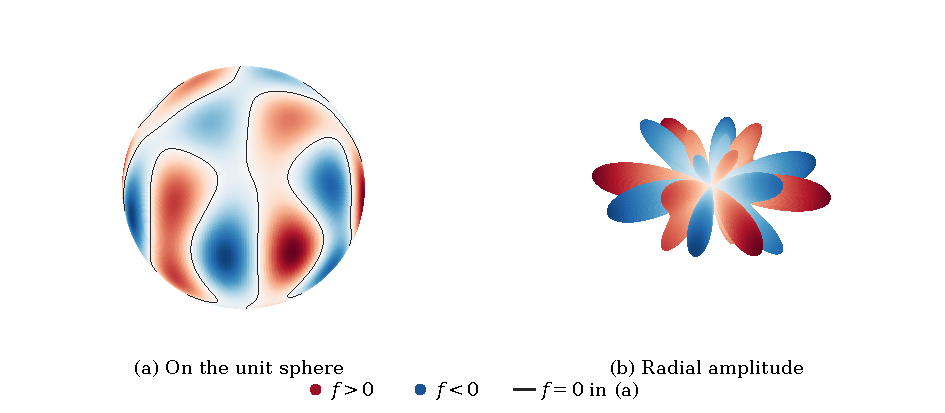
\includegraphics[width=0.97\textwidth]{figures/spherical_harmonic_panels.pdf}
\caption{A degree-six spherical harmonic \(f=\Phi|_{\Sph^2}\), where
\(\Phi=\operatorname{Re}((x+iy)^6+\tfrac12(y+iz)^6+
\tfrac13(z+ix)^6)\). Left: values on the unit sphere, with the nodal
set in black. Right: the radial amplitude plot
\(\theta\mapsto c^{-1}|f(\theta)|\theta\), with a positive display
normalization \(c\). Red and blue indicate positive and negative values.
The link of the zero cone is the nodal set in the left panel.
Visualization inspired by Matthew de Courcy-Ireland's illustration in
Logunov's lecture slides \cite[slide~4]{Logunov2020}.}
\label{fig:spherical-harmonic}
\end{figure}

\begin{proposition}[Irreducible effective equations for minimizing cones]
\label{prop:minimizing-irreducibility}
Let \(F\in\R[x_1,\ldots,x_N]\), \(N\ge2\), be nonconstant,
homogeneous and square-free. Suppose \(E=\{F<0\}\) is locally
perimeter minimizing in \(\R^N\) and
\(\partial\llbracket E\rrbracket\ne0\).
Then exactly one real irreducible factor of \(F\) has a nonsingular
real zero. After absorbing a nonzero constant and signs into this
factor, one can write
\[
\begin{gathered}
 F=PQ,\qquad P\text{ real irreducible},\qquad Q\ge0,\\
 \{F<0\}=\{P<0\}\quad\text{almost everywhere}.
\end{gathered}
\]
In particular, if every real irreducible factor has a nonsingular
real zero, then \(F\) is irreducible. Under the same minimizing
hypotheses, harmonic \(F\) is therefore irreducible.
\end{proposition}

\begin{proof}
Let \(V=|\partial\llbracket E\rrbracket|\) and
\(M=\operatorname{reg}V\). Its nonempty support is a closed cone,
hence connected. Regularity of minimizing boundaries makes \(M\)
real analytic and gives \(\cH^{N-2}(\operatorname{sing}V)=0\)
\cite[Part~III, introductory theorem, pp.~275--277]{Maggi12}.
Thus \(M\) is connected: for \(N=2\) this follows from smoothness,
and for \(N\ge3\) from
\cite[Section~5, proof of Theorem~1.1; Theorem~3.2]{WickramasekeraMaximum14}.
The singular set here belongs to the boundary, not to its polynomial
representation.

We use the following elementary divisibility fact. If a polynomial
\(H\) vanishes on a nonempty smooth open patch of the zero set of
a real irreducible polynomial \(P_j\), then \(P_j\mid H\).
Indeed, express the patch as a graph \(t=\varphi(x')\).
If \(P_j\nmid H\), Gauss' lemma
\cite[Chapter~VIII, Section~5]{Knapp16} makes \(P_j,H\) coprime over
\(\R(x')\), so their resultant in \(t\) is a nonzero polynomial
in \(x'\). The common root \(\varphi(x')\) makes it vanish on
an open set, a contradiction.

Write \(F=c\prod_jP_j\) with distinct irreducible factors.
For each factor with a nonsingular real zero, the divisibility fact
and coprimality give a nonempty smooth patch
\(U_j\subset\{P_j=0\}\) avoiding all other factors. On \(U_j\),
\(\nabla F\ne0\) and \(F\) changes sign, so \(U_j\subset M\).
If two such factors \(P_1,P_2\) existed, the analytic function
\(P_1|_M\), zero on \(U_1\), would vanish on connected \(M\),
contradicting \(P_1\ne0\) on \(U_2\).

For an irreducible real polynomial, having a nonsingular real zero
is equivalent to changing sign
\cite[Theorem~4.5.1]{BochnakCosteRoy98}. There must be one such
factor, since otherwise \(F\) is of fixed sign and
\(\partial\llbracket E\rrbracket=0\). Choose the signs of the
remaining factors to make their product \(Q\ge0\).
Its zero set is Lebesgue null, proving equality of the phases almost
everywhere. The harmonic assertion follows from
\cref{lem:square-free-critical-set}.
\end{proof}

\begin{example}[A redundant line and two intersecting hyperplanes]
\label{rem:reducible-minimal-equations}
For \(F=x(y^2+z^2)\) in \(\R^3\), the zero set is the plane
\(P=\{x=0\}\) together with the line \(\ell=\{y=z=0\}\).
The negative phase agrees almost everywhere with \(\{x<0\}\);
its boundary current is the plane calibrated by \(dy\wedge dz\),
with support \(P\). The extra line contributes no two-dimensional mass.
For \(F=xy\), instead, \(\Delta F=0\) and \(\cL(F)=-2F\),
so the regular zero set is minimal, but both factors contribute
hypersurface branches. Their boundary is not area minimizing by
\cref{prop:minimizing-irreducibility}. For the elementary crossing-lines
comparison and its product with a line, see
\cite[Figures~10.1.3 and~10.7.1, Lemma~10.6]{Morgan16}.
See also the regularity
obstruction in \cite[Theorem~28.1]{Maggi12} and
\cite[Section~1 and Theorem~1]{Federer70}.
\end{example}

\begin{figure}[htbp]
\centering
% Two schematic zero sets in R^3.  All conclusions concern 2-dimensional currents.
% The transverse line in the left panel is not part of the current support.
\begingroup
\centering
\resizebox{\linewidth}{!}{%
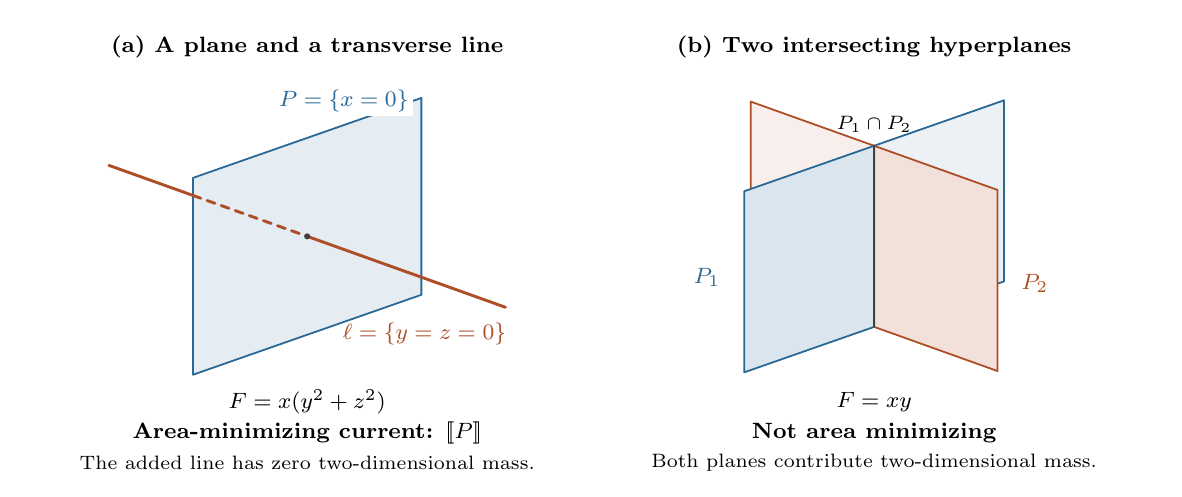
\begin{tikzpicture}[x=1cm,y=1cm,line cap=round,line join=round,
  font=\footnotesize]
  \definecolor{coneplane}{RGB}{42,104,149}
  \definecolor{coneline}{RGB}{173,78,39}
  \tikzset{plane edge/.style={draw=coneplane,line width=.65pt},
    second edge/.style={draw=coneline,line width=.65pt}}
  % The fixed bounding box makes the two panels equally wide.
  \path[use as bounding box] (-3.55,-2.95) rectangle (10.75,2.65);

  \begin{scope}
    \node[font=\footnotesize\bfseries] at (0,2.4)
      {(a) A plane and a transverse line};
    % P={x=0}; projected y- and z-directions are (1,.35) and (0,1).
    \filldraw[plane edge,fill=coneplane!12]
      (-1.45,-1.7575)--(1.45,-.7425)--(1.45,1.7575)--(-1.45,.7425)--cycle;
    % The x-axis has projected direction (.95,-.34).  Its rear segment is
    % dashed precisely where it lies behind the displayed patch of P.
    \draw[coneline,line width=1.05pt] (-2.5175,.901)--(-1.45,.51895);
    \draw[coneline,line width=1.05pt,dash pattern=on 3pt off 2.4pt]
      (-1.45,.51895)--(0,0);
    \draw[coneline,line width=1.05pt] (0,0)--(2.5175,-.901);
    \fill[black!75] (0,0) circle (1.1pt);
    \node[coneplane,anchor=south east,fill=white,inner sep=1.6pt]
      at (1.35,1.52) {$P=\{x=0\}$};
    \node[coneline,anchor=north east] at (2.65,-.98)
      {$\ell=\{y=z=0\}$};
    \node at (0,-2.1) {$F=x(y^2+z^2)$};
    \node[font=\footnotesize\bfseries] at (0,-2.5)
      {Area-minimizing current: $[\![P]\!]$};
    \node[font=\scriptsize] at (0,-2.87)
      {The added line has zero two-dimensional mass.};
  \end{scope}

  \begin{scope}[xshift=7.2cm]
    \node[font=\footnotesize\bfseries] at (0,2.4)
      {(b) Two intersecting hyperplanes};
    % P_1={x=0}, P_2={y=0}.  Draw the rear half-planes first, then the
    % front half-planes, so both sheets and their intersection are visible.
    \filldraw[plane edge,fill=coneplane!9]
      (0,-1.15)--(1.65,-.5725)--(1.65,1.7275)--(0,1.15)--cycle;
    \filldraw[second edge,fill=coneline!9]
      (-1.5675,-.589)--(0,-1.15)--(0,1.15)--(-1.5675,1.711)--cycle;
    \filldraw[plane edge,fill=coneplane!17]
      (-1.65,-1.7275)--(0,-1.15)--(0,1.15)--(-1.65,.5725)--cycle;
    \filldraw[second edge,fill=coneline!17]
      (0,-1.15)--(1.5675,-1.711)--(1.5675,.589)--(0,1.15)--cycle;
    \draw[black!75,line width=.9pt] (0,-1.15)--(0,1.15);
    \node[coneplane,anchor=east] at (-1.83,-.52) {$P_1$};
    \node[coneline,anchor=west] at (1.75,-.6) {$P_2$};
    \node[anchor=south,font=\scriptsize] at (0,1.2) {$P_1\cap P_2$};
    \node at (0,-2.1) {$F=xy$};
    \node[font=\footnotesize\bfseries] at (0,-2.5)
      {Not area minimizing};
    \node[font=\scriptsize] at (0,-2.87)
      {Both planes contribute two-dimensional mass.};
  \end{scope}
\end{tikzpicture}
}
\par
\endgroup

\caption{Left: \(\{x(y^2+z^2)=0\}=P\cup\ell\), but the minimizing
boundary current has support \(P\). Right: both intersecting
hyperplanes in \(\{xy=0\}\) carry area; their union is stationary
as a varifold but the associated boundary current is not area minimizing.
Both pictures are illustrated in \(\R^3\).}
\label{fig:reducible-cones}
\end{figure}

\phantomsection\label{par:irreducible-convention}
For structural results, unless stated otherwise, we choose a nonconstant
real homogeneous irreducible defining polynomial with \(C_{\reg}\ne\varnothing\).
Removing a nonnegative factor preserves the boundary current, but may
change the full zero set, the degree and \(\cA_R(F)\); all degree
and generator statements refer to the chosen effective equation.

\Needspace{12\baselineskip}
The classical algebraic minimality criterion now takes the following
form; see \cite[Section~6.2.1, equation~(6.2.2)]{NadirashviliTkachevVladut14}.

\begin{proposition}[Minimality and polynomial divisibility]
\label{prop:divisibility}
Let \(F\) be real irreducible and homogeneous of degree \(e\ge1\),
with \(C_{\reg}\ne\varnothing\). Then \(C_{\reg}\) is minimal
if and only if
\begin{equation}\label{eq:L-divisibility}
 \cL(F)=F\lambda_F,
\end{equation}
where \(\lambda_F\) is homogeneous of degree \(2e-4\), possibly
zero, for \(e\ge2\), and \(\lambda_F=0\) for \(e=1\).
The same equivalence holds for a square-free homogeneous \(F\)
when every real irreducible factor has a nonsingular real zero.
\end{proposition}

\begin{proof}
By \eqref{eq:div-normalized-gradient}, minimality means
\(\cL(F)=0\) on \(C_{\reg}\). The patch divisibility argument
in \cref{prop:minimizing-irreducibility} gives \(F\mid\cL(F)\).
For the square-free extension, take for each factor a nonsingular
patch avoiding the others, apply the same argument, and use
pairwise coprimality. Since \(\deg\cL(F)=3e-4\) when it is
nonzero, the degree follows. For \(e=1\), all second derivatives
vanish. The converse follows from the same curvature formula.
\end{proof}

The factor condition cannot be omitted in the square-free extension:
for \(t=y^2+z^2\) and \(F=x(2x^2+t)\), the regular zero set is
planar, but
\(\cL(F)=8(9x^2-t)F+4xt^2\) is not divisible by \(F\).
Its effective equation is simply \(x\).

Under \eqref{eq:L-divisibility}, differential closure and polynomial
division \cite[Lemma~24(b)]{MendesRadeschi}, or
\cref{prop:MR-finite-and-division}, give \(\lambda_F\in\cA_R(F)\).
In the harmonic case this becomes
\begin{equation}\label{eq:harmonic-minimal-weight}
 \Delta F=0,\qquad S=|\nabla F|^2,\qquad
 \Gamma(F,S)=2qF,\qquad q=-\lambda_F,
\end{equation}
with \(S,q\in\cA_R(F)\). These identities simplify the closure
calculation, while \cref{prop:uniform-finite-generation} supplies the
uniform generator bound.
